\section{Símbolos discretos y filtros A--F}

El algoritmo anterior queda determinado por el símbolo $\tau$ usado para construir el multiplicador discreto $M_\tau$. En esta sección se describen los siete símbolos evaluados: la rampa como referencia y seis filtros exploratorios, denotados A--F.

\subsection*{Rampa de referencia}

El símbolo de referencia es la rampa canónica
\[
\tau_{\mathrm{rampa}}(\sigma)=|\sigma|.
\]
Esta elección corresponde directamente a la fórmula continua de FBP fijada en el Capítulo 2. En la implementación discreta no se introduce ningún factor adicional en este símbolo.

\subsection*{Filtros exploratorios A, B y C}

El filtro A modifica la rampa mediante una perturbación oscilatoria dependiente de la frecuencia:
\[
\tau_A(\sigma)
=
|\sigma|\left(1+\frac{\sin|\sigma|}{1+|\sigma|}\right).
\]
El filtro B tiene respuesta no nula en frecuencia cero:
\[
\tau_B(\sigma)=\sqrt{0.3^2+|\sigma|^2}.
\]
En particular, $\tau_B(0)=0.3$. En cambio, la rampa y los filtros A, C, D, E y F se anulan en frecuencia cero.\\

El filtro C introduce un corte compacto relativo a la frecuencia máxima de la grilla discreta:
\[
\tau_C(\sigma)
=
|\sigma|\left(1-\frac{|\sigma|}{\sigma_c}\right)_+,
\qquad
\sigma_c=0.6\sigma_{\max}.
\]
Aquí $(a)_+=\max\{a,0\}$.

\subsection*{Filtros D, E y F}

Los filtros D, E y F crecen como la rampa hasta $|\sigma|=20$ y luego modifican el tratamiento de frecuencias mayores. El filtro D es triangular:
\[
\tau_D(\sigma)=
\begin{cases}
|\sigma|, & |\sigma|\le 20,\\
40-|\sigma|, & 20<|\sigma|\le 40,\\
0, & |\sigma|>40.
\end{cases}
\]
El filtro E usa decaimiento exponencial moderado:
\[
\tau_E(\sigma)=
\begin{cases}
|\sigma|, & |\sigma|\le 20,\\
20\exp[-0.08(|\sigma|-20)], & |\sigma|>20.
\end{cases}
\]
El filtro F usa decaimiento exponencial más rápido:
\[
\tau_F(\sigma)=
\begin{cases}
|\sigma|, & |\sigma|\le 20,\\
20\exp[-0.50(|\sigma|-20)], & |\sigma|>20.
\end{cases}
\]

Estos seis filtros no se presentan como filtros óptimos. Su propósito es explorar, bajo una misma configuración numérica, cómo distintas respuestas espectrales alteran la reconstrucción y su sensibilidad al ruido. Esta pregunta se relaciona con el análisis de error y el diseño de funciones filtro en FBP \cite{beckmann_iske2017,beckmann_nickel2025}, pero los símbolos A--F usados aquí no se derivan de esos trabajos ni reproducen sus filtros optimizados.

La Figura~\ref{fig:chapter3-symbols} muestra la rampa y los filtros A--F sobre la grilla de frecuencias usada por la DFT.

\begin{figure}[htbp]
    \centering
    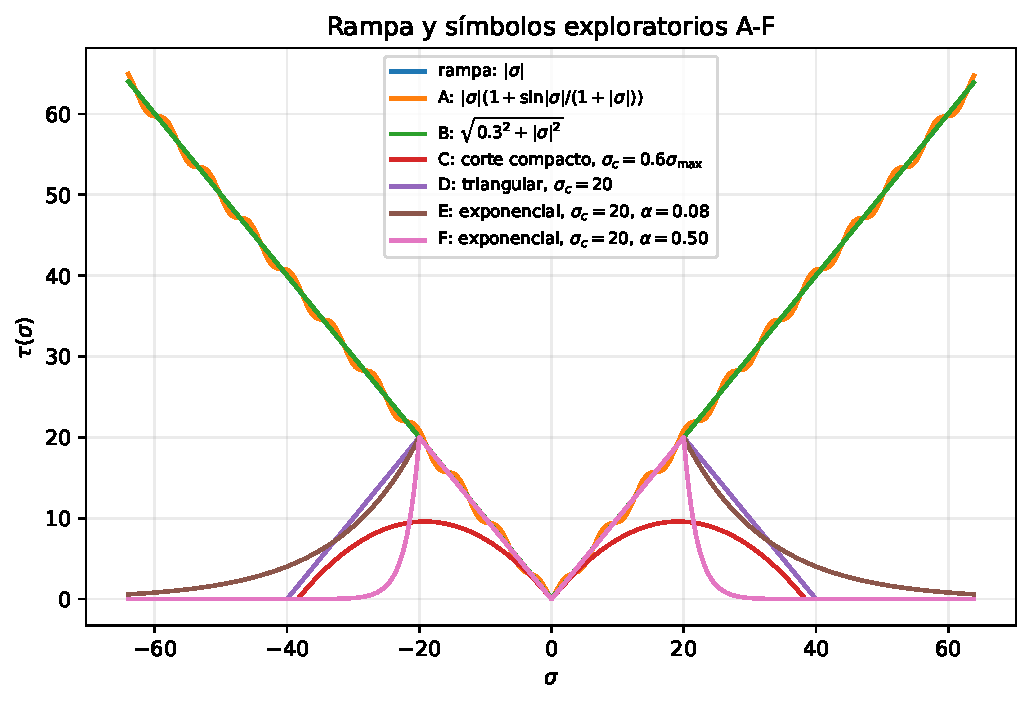
\includegraphics[width=0.86\textwidth]{Figures/Chapter3/symbols_ramp_A_F.pdf}
    \caption{Símbolos discretos evaluados sobre la grilla de frecuencias de longitud $N_{\mathrm{fft}}=1024$. La rampa se usa como referencia; los símbolos A--F son filtros exploratorios para estudiar el efecto de distintas modificaciones espectrales.}
    \label{fig:chapter3-symbols}
\end{figure}
